\documentclass[10pt]{article}
\usepackage[margin=1in]{geometry}
\usepackage[T1]{fontenc}
\usepackage{amsmath,amssymb}
\usepackage{graphicx}
\usepackage{booktabs}
\usepackage{caption}
\usepackage[hidelinks]{hyperref}

\graphicspath{{../assets/}}

\title{SceneCast: A Laptop-Scale Vectorized Scene Transformer for Motion Forecasting,\\
and a Dropout-Induced Mode Collapse in Winner-Takes-All Decoders}
\author{Hritvik Hooda}
\date{November 2026}

\begin{document}
\maketitle

\begin{abstract}
In this paper, we present SceneCast, a 1.6M parameter vectorized scene transformer for
multimodal motion forecasting which trains on a laptop. Each agent trajectory and each lane
centerline is represented by a single token, a transformer mixes the tokens, and six queries
are used to generate six candidate futures with associated confidences, with a
winner-takes-all loss objective. Training on 20{,}000 scenes (10\% of the Argoverse~2 Motion
Forecasting training dataset), and evaluating on 3{,}000 validation scenes, it achieves
minADE$_6$ = 1.06\,m, minFDE$_6$ = 2.07\,m and a miss rate of 0.32, compared to 4.75\,m,
12.25\,m and 0.87 for a constant velocity baseline. Ablations reveal that excluding the lane
map increases minFDE$_6$ by 35\%, and that excluding the surrounding agents increases it by
4\%. Additionally, we report a failure mode that we observed when training our model: with
near identical mode-query initialization and dropout in the decoder, winner-takes-all
training can lead the model to rely on the noise created by dropout as the source of
diversity between the modes. The modes will thus be distinct during training, but collapse
at test time. This failure mode is investigated experimentally on a synthetic multimodal
prediction task. This is a technical report on a reimplementation on a small scale, not a
novel state-of-the-art model; code is available at
\url{https://github.com/hritvikhooda11/scenecast}.
\end{abstract}

\section{Introduction}

Motion prediction, estimating the future locations of surrounding agents over the next few
seconds, is naturally multimodal, since an agent approaching an intersection might choose to
go left, right, or straight, with history observations typically unable to distinguish
between those choices. The modern approach is to estimate a small set of potential paths with
associated probabilities, while publicly available benchmarks like
Argoverse~2~\cite{wilson2021argoverse2} and the Waymo Open Motion
Dataset~\cite{ettinger2021womd} score the best of $K$ candidates.

Since VectorNet~\cite{gao2020vectornet}, the most prevalent approach to date has been
modeling the scene as polylines (trajectories of agents and features of the map), as opposed
to rasterizing it into an image, and processing the tokens thusly generated with
attention~\cite{vaswani2017attention,liang2020lanegcn,ngiam2022scenetransformer,
nayakanti2023wayformer,zhou2022hivt,shi2022mtr,zhou2023qcnet}. The state-of-the-art models
from this category have been trained on the full datasets.

The present paper poses a more specific and practical question: How far will a minimalist
version of this approach get with a laptop and an order of magnitude less data, and where do
things break? Our contributions are small:
\begin{itemize}
  \item A compact implementation (Section~\ref{sec:method}) and experiments, ablations, and
        failure analysis on a smaller subset of Argoverse~2
        (Sections~\ref{sec:results} and~\ref{sec:failures}).
  \item A discussion and controlled demonstration of a mode collapse failure where a
        ``winner takes all'' decoder uses dropout noise to distinguish between its modes
        (Section~\ref{sec:collapse}). While we haven't seen the specific interaction
        discussed in any of the cited literature, we have not performed a comprehensive
        literature review, and it may already be well-known among practitioners.
\end{itemize}

\section{Related work}

\paragraph{Vectorized scene encoding.} The polylines in VectorNet~\cite{gao2020vectornet} are
encoded using a subgraph similar to PointNet~\cite{qi2017pointnet}, while the relations
between polylines are modeled with global attention. LaneGCN~\cite{liang2020lanegcn} uses the
lane graph. Scene Transformer~\cite{ngiam2022scenetransformer},
Wayformer~\cite{nayakanti2023wayformer}, HiVT~\cite{zhou2022hivt}, MTR~\cite{shi2022mtr}, and
QCNet~\cite{zhou2023qcnet} learn attention-based encoder-decoder models with different design
choices of the coordinate frame and the queries. SceneCast is most similar to a small
VectorNet encoder with a DETR-like~\cite{carion2020detr} learned-query decoder.

\paragraph{Multimodal outputs and mode collapse.} Using multiple output heads, such that only
the best one is penalized, dates back to multiple choice learning~\cite{guzman2012mcl} and is
a common practice for trajectory prediction~\cite{cui2019mtp}. This approach is well-known to
be sensitive to initialization, where either some of the hypotheses are never selected at
all, or all of them become identical. In order to relax the assignment, the evolving
winner-takes-all mechanism~\cite{makansi2019ewta} is sometimes employed. There are other
solutions that avoid modes of arbitrary shape, using trajectory anchors in
MultiPath~\cite{chai2019multipath} or goal points on the map in TNT~\cite{zhao2020tnt} and
DenseTNT~\cite{gu2021densetnt}. Our failure case described in Section~\ref{sec:collapse}
represents a different way of collapsing: during training the hypotheses are diverse, but for
a reason that disappears at evaluation time.

\section{Method}
\label{sec:method}

\subsection{Scene representation}

The task follows the Argoverse~2 protocol: 5\,s of history and 6\,s of future at 10\,Hz for a
designated focal agent, so $T_\text{obs}=50$ and $T_\text{fut}=60$ steps.

\paragraph{Focal-centric frame.} Every scene is translated and rotated so that the focal agent
is at the origin with heading along $+x$ at the last observed step. All positions, headings
and velocities of all agents and all lane points are expressed in this frame.

\paragraph{Agents.} We keep the focal agent and the 31 nearest other agents that are observed
at the last history step ($N=32$). Each agent is a polyline of 50 points with features
$(x, y, \cos\psi, \sin\psi, v_x, v_y)$, a normalised time stamp in $[-1, 0]$ and a validity
bit. Positions are divided by 50 and velocities by 10 before encoding. Each agent also
carries one of ten object-type labels following the Argoverse~2 taxonomy; static, background
and construction objects are kept as agents with their own type embeddings.

\paragraph{Map.} We use lane centerlines only. Each lane segment is resampled to 10 points
evenly spaced by arc length, and the $M=96$ segments nearest to the focal agent within 120\,m
are kept. Point features are $(x, y, \Delta x, \Delta y)$ and a flag for whether the segment
lies inside an intersection.

\subsection{Architecture}

\paragraph{Polyline encoder.} Agents and lanes use separate encoders of the same form: a
point-wise MLP, a masked max-pool over the points of the polyline, concatenation of the pooled
vector back onto every point, a second MLP and a second masked max-pool, giving one
$d$-dimensional token per polyline ($d=128$). Agent tokens receive a learned type embedding,
and all tokens receive a learned embedding marking them as the focal agent, another agent or
a lane.

\paragraph{Scene encoder.} The $N+M=128$ tokens are processed by four pre-norm transformer
encoder layers~\cite{vaswani2017attention} with 8 heads, feed-forward width 512 and dropout
0.1, with padding masks for absent agents and lanes.

\paragraph{Mode decoder.} $K=6$ learned query vectors, each added to a linear projection of
the encoded focal-agent token, pass through two pre-norm transformer decoder layers that
cross-attend to the scene tokens. An MLP head maps each output to $T_\text{fut}$ per-step
displacements, whose cumulative sum is the predicted trajectory, and a second head produces a
confidence logit. In the final model the queries are initialised from $\mathcal{N}(0, 1)$ and
the decoder has no dropout; Section~\ref{sec:collapse} explains why. The model has 1.56M
parameters.

\subsection{Training}

Let $\hat{\mathbf{y}}^{(k)}$ be the $k$-th predicted trajectory, $\mathbf{y}$ the ground truth
and $k^\star$ the mode with the lowest average displacement error. The loss is
\begin{equation}
\mathcal{L} = \frac{1}{T}\sum_{t=1}^{T} \ell_{\text{Huber}}\!\left(\hat{\mathbf{y}}^{(k^\star)}_t,
\mathbf{y}_t\right) - \log \operatorname{softmax}(\mathbf{c})_{k^\star},
\end{equation}
where $\ell_{\text{Huber}}$ is the smooth-$L_1$ loss summed over the two coordinates,
$\mathbf{c}$ are the confidence logits, and the average runs over valid future steps. Only the
winning mode receives a regression gradient.

We train with AdamW~\cite{loshchilov2019adamw} (learning rate $5\times10^{-4}$, weight decay
$10^{-2}$), batch size 64, 500 steps of linear warm-up followed by cosine decay, and gradient
clipping at norm 5, for 40 epochs. No data augmentation is used.

\section{Experiments on Argoverse 2}
\label{sec:results}

\paragraph{Data.} We use the first 20{,}000 scenarios of the Argoverse~2 Motion
Forecasting~\cite{wilson2021argoverse2} training split and the first 3{,}000 of the validation
split, in the lexicographic order of scenario identifiers; this is 10\% of the training data
and 12\% of the validation data.

\paragraph{Metrics.} Following the benchmark, minADE$_6$ and minFDE$_6$ are the average and
final displacement errors of the best of the six modes, the miss rate (MR) is the fraction of
scenes where the best mode ends more than 2\,m from the truth, and brier-minFDE$_6$ adds
$(1-p)^2$ to minFDE$_6$, where $p$ is the confidence of the best mode. We also report
minFDE$_1$, the final error of the single most confident mode.

\paragraph{Compute.} All runs used the GPU of an Apple M4 laptop with 24\,GB of memory. The
three models in Table~\ref{tab:results} were trained concurrently on that one machine and each
took about 3.5 hours under that sharing.

\begin{table}[t]
\centering
\caption{Results on 3{,}000 Argoverse~2 validation scenarios after training on 20{,}000
scenarios. Lower is better. Distances in metres.}
\label{tab:results}
\begin{tabular}{lccccc}
\toprule
Model & minADE$_6$ & minFDE$_6$ & MR & brier-minFDE$_6$ & minFDE$_1$ \\
\midrule
Constant velocity (one mode) & 4.75 & 12.25 & 0.865 & 12.25 & 12.25 \\
SceneCast                    & \textbf{1.06} & \textbf{2.07} & \textbf{0.324} & \textbf{2.71} & \textbf{6.65} \\
\quad without map            & 1.30 & 2.79 & 0.422 & 3.41 & 7.86 \\
\quad without other agents   & 1.08 & 2.15 & 0.361 & 2.78 & 7.34 \\
\bottomrule
\end{tabular}
\end{table}

\begin{figure}[t]
\centering
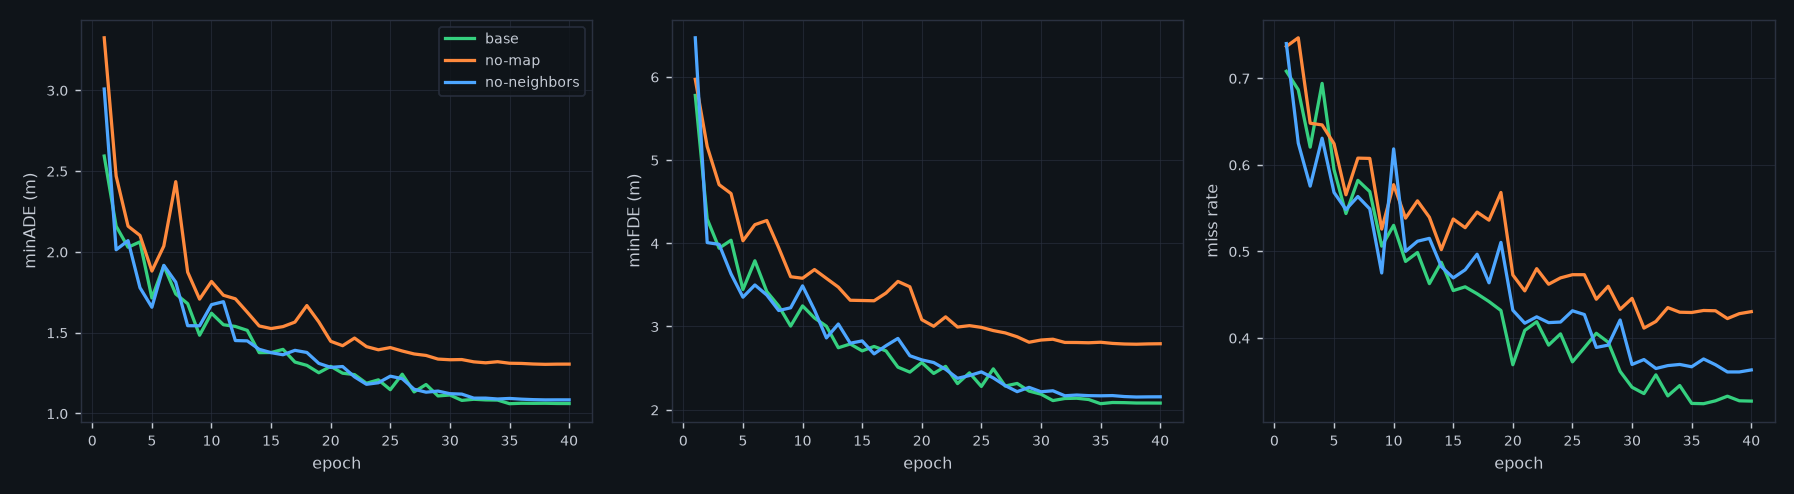
\includegraphics[width=\linewidth]{curves.png}
\caption{Validation metrics during training for the full model and the two ablations.}
\label{fig:curves}
\end{figure}

\begin{figure}[t]
\centering
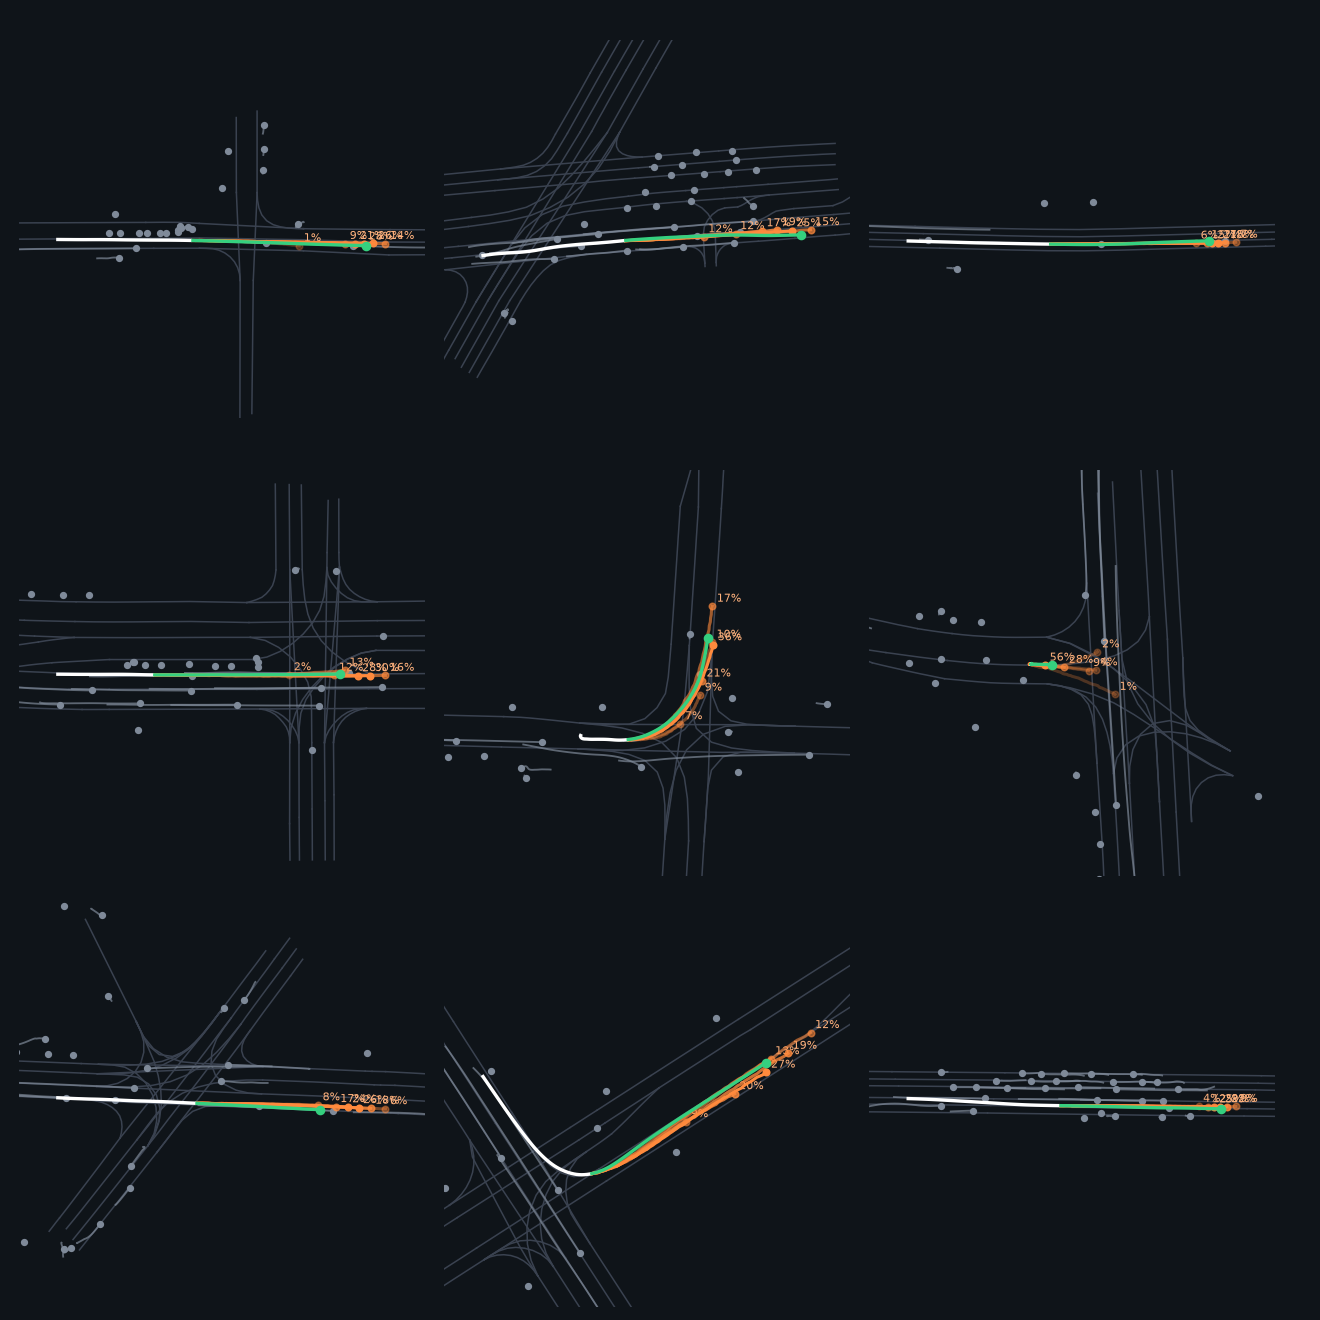
\includegraphics[width=0.8\linewidth]{grid.png}
\caption{Predictions on nine consecutive validation scenes. White: observed history. Green:
ground-truth future. Orange: the six predicted modes with their confidences. Grey: lane
centerlines and other agents.}
\label{fig:grid}
\end{figure}

\paragraph{Results.} Table~\ref{tab:results} and Figure~\ref{fig:curves} summarise the
results; Figure~\ref{fig:grid} shows typical predictions. SceneCast reduces minFDE$_6$ from
12.25\,m to 2.07\,m relative to constant velocity.

\paragraph{Ablations.} The two ablations mask the corresponding tokens out of attention and
are otherwise trained identically. Without the map, minFDE$_6$ rises by 35\% (2.07 to 2.79\,m)
and the miss rate from 0.324 to 0.422; the gap appears within the first few epochs and
persists. Without other agents, minFDE$_6$ rises by only 4\%, while the miss rate rises from
0.324 to 0.361 and minFDE$_1$ from 6.65 to 7.34\,m. One reading is that, at this scale,
surrounding agents contribute more to ranking the candidate futures than to generating them,
but with one seed per configuration this difference should be treated as suggestive.

\paragraph{Confidence.} The gap between minFDE$_6$ (2.07\,m) and minFDE$_1$ (6.65\,m) shows
that the confidence head is the weakest part of the model: a good candidate usually exists
among the six but is often not ranked first.

\paragraph{Caveats.} Each configuration was run once. The checkpoint reported for each run is
the one with the lowest validation minFDE$_6$ on the same 3{,}000 scenarios used for
reporting, which biases the numbers slightly downward. Because of the reduced training set and
the validation subset, these numbers are not comparable with the public leaderboard, where
methods trained on the full data, such as QCNet~\cite{zhou2023qcnet}, report substantially
lower errors.

\section{Failure analysis}
\label{sec:failures}

\begin{figure}[t]
\centering
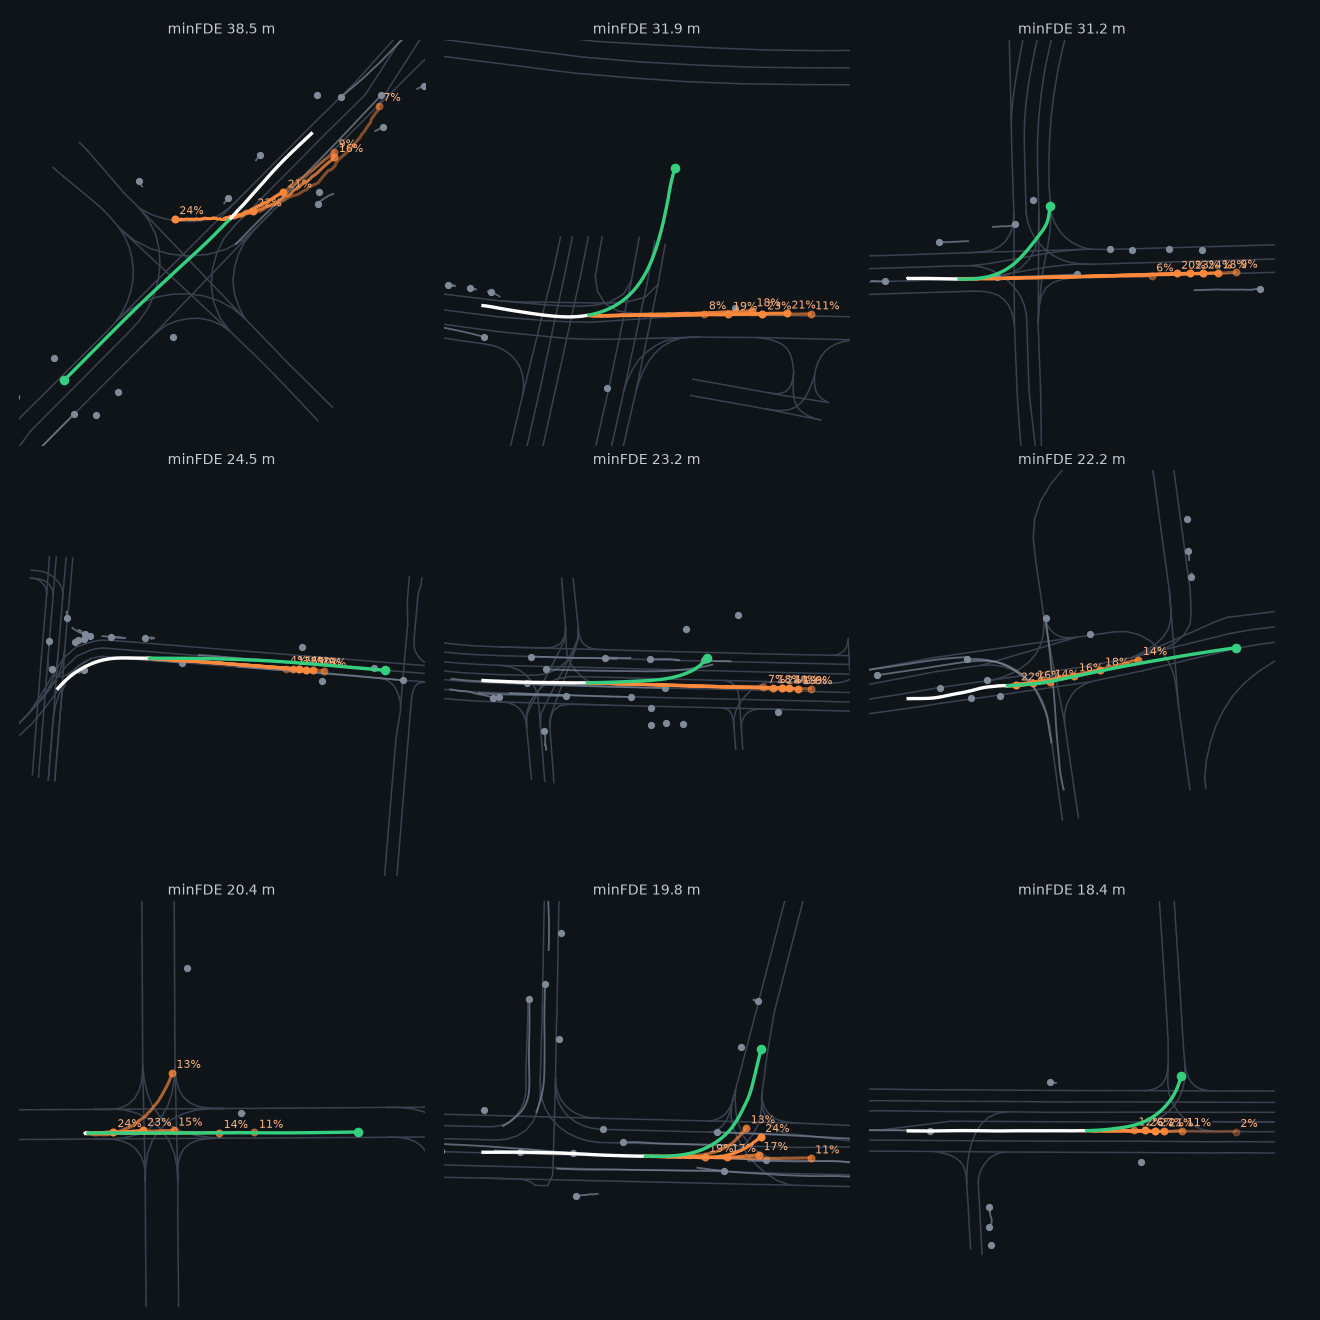
\includegraphics[width=0.8\linewidth]{failures.png}
\caption{The nine scenes with the highest minFDE$_6$ among the first 2{,}000 validation
scenes.}
\label{fig:failures}
\end{figure}

Figure~\ref{fig:failures} shows the nine worst scenes among the first 2{,}000 validation
scenes. By inspection they fall into three groups.

\paragraph{Missed turns (five scenes).} The agent turns or changes lane and all or nearly all
of the six modes continue straight. In these and in typical scenes (Figure~\ref{fig:grid}),
the modes are spread along the direction of travel, differing in speed, rather than across
manoeuvres. A plausible explanation is that most training futures are approximately straight,
so under winner-takes-all assignment the queries specialise in the dimension that most often
reduces error, namely speed.

\paragraph{Wrong speed profile (three scenes).} The path is correct, but the agent travels
much further than any mode predicts, for example when pulling away after a turn.

\paragraph{Wrong direction (one scene).} The predictions run opposite to the true direction
of travel. We have not determined the cause; an unreliable heading estimate for a slow-moving
agent, which would corrupt the focal-centric frame, is one candidate.

The first group suggests anchoring modes to the map, by proposing goal points on reachable
lanes and decoding one trajectory per goal~\cite{zhao2020tnt,gu2021densetnt}, in place of
free-form learned queries.

\section{Dropout-induced mode collapse}
\label{sec:collapse}

\subsection{Observation}

An earlier version of the decoder differed from the final one in two ways: the mode queries
were initialised from $\mathcal{N}(0, 0.02^2)$, and the decoder layers used dropout 0.1 like
the encoder. On the synthetic task described below, this version trained normally, with a
steadily falling loss, yet its validation metrics (computed with dropout disabled, as usual)
were poor and all six predicted modes were nearly identical. Evaluating the same weights with
dropout left on gave far better numbers. The model had learned diverse modes, but the
diversity came from the dropout masks rather than from the queries.

The mechanism we propose is as follows. With near-identical queries, the $K$ decoder outputs
start out near-identical and winner-takes-all assignment has nothing to separate. Dropout is
sampled independently for each query position, so it perturbs the $K$ outputs differently.
The regression loss only rewards the closest output, so the network can reduce its loss by
amplifying those perturbations into large differences between trajectories, in effect turning
the decoder into a sampler driven by dropout noise. Nothing in the objective requires the
diversity to be tied to the query identity, so at evaluation time, when the noise is removed,
the outputs coincide.

\subsection{Controlled study}

\paragraph{Synthetic task.} To study this in isolation we use a generator of four-way
intersection scenes. The focal vehicle is 5 to 40\,m before the intersection at the prediction
time and proceeds left, straight or right along a lane-following path, so the future is
multimodal by construction; 3 to 11 other vehicles follow other routes. Scenes are randomly
rotated and translated and pass through the same preprocessing as the real data. We use 6{,}000
training and 800 validation scenes.

\paragraph{Design.} We train the same model for 20 epochs in a $2\times2$ design, crossing the
query initialisation scale ($0.02$ or $1$) with decoder dropout ($0.1$ or $0$), with two seeds
per cell. Each final checkpoint is evaluated twice on the validation set: with dropout
disabled (evaluation mode) and with dropout enabled (training mode). We report minFDE$_6$ and
the \emph{spread}, the mean pairwise distance between the six predicted endpoints.

% PLACEHOLDER: generated from results/collapse_study.json once the eight runs finish.
\begin{center}\textit{[Table: results of the $2\times2$ study, pending completion of the runs.]}\end{center}


\subsection{Discussion}

% PLACEHOLDER: to be written from the study results.
\textit{[Discussion pending the results of the study.]}


\section{Limitations}

Beyond the caveats in Section~\ref{sec:results}: the model predicts a single focal agent
rather than joint futures; it uses lane centerlines only, without crosswalks, lane boundaries
or traffic-light state; it uses a single focal-centric frame, so tokens far from the focal
agent are encoded in a frame that is not natural for them; and the collapse study uses a
synthetic task with a small number of seeds, so it establishes that the failure can occur and
which factors produce it in this setting, not how common it is in larger models or on real
data.

\section{Conclusion}

A minimal vectorized scene transformer trained on a laptop with a tenth of Argoverse~2 already
captures most of the benefit over a kinematic baseline, with the lane map contributing far
more than surrounding agents at this scale, and its dominant failure is a lack of
manoeuvre-level diversity among modes. Separately, we find that dropout inside a
winner-takes-all query decoder can silently become the source of mode diversity. The practical
recommendations are to initialise mode queries at a scale that makes them distinct, to be
cautious with dropout on the path from queries to outputs, and to compare training-mode and
evaluation-mode metrics when multimodal predictions look collapsed.

\section*{Acknowledgements}

The author used Claude Fable 5.2 (Anthropic), an AI assistant, as a tool during this work for
help with code development, running experiments and drafting the manuscript. The author
reviewed and verified the results and takes full responsibility for the content of this
report.

\bibliographystyle{plain}
\bibliography{references}

\end{document}
